\documentclass[10pt,sans,english,compress,xcolor=dvipsnames]{beamer}
\author[Lily ]{ Dr Lily Asquith (Lily, she/her)}

\usetheme{Szeged}
%\defbeamertemplateparent{enumerate items}{enumerate item,enumerate subitem,enumerate subsubitem,enumerate mini template}
\definecolor{titcol}{RGB}{16,78,100} 
\setbeamercolor{frametitle}{fg=titcol,bg=White}
\useoutertheme{miniframes} 
\useinnertheme{rectangles}

\usepackage{pifont}
\newcommand{\tick}{\textcolor{grn}{\ding{52} } }
\newcommand{\nope}{\textcolor{red}{\ding{54} } }


\usepackage{soul}
\usepackage{cancel}

\usepackage[most]{tcolorbox}
\definecolor{LilyBlack}{rgb}{0.05,0.1,0.3} % UBC Blue (primary)
\usecolortheme[named=LilyBlack]{structure}

\usepackage{booktabs}
\usepackage{tabularx}
%\usepackage{tikz}
%\def\checkmark{\tikz\fill[scale=0.4](0,.35) -- (.25,0) -- (1,.7) -- (.25,.15) -- cycle;}

\usepackage{physics}

\usepackage{xparse}

\setbeamertemplate{footline}{%
  \leavevmode%
  \hbox{\begin{beamercolorbox}[wd=.5\paperwidth,ht=2.5ex,dp=1.125ex,leftskip=.3cm plus1fill,rightskip=.3cm]{author in head/foot}%
    \usebeamerfont{author in head/foot}\insertshortauthor
  \end{beamercolorbox}%
  \begin{beamercolorbox}[wd=.5\paperwidth,ht=2.5ex,dp=1.125ex,leftskip=.3cm,rightskip=.3cm plus1fil]{title in head/foot}%
    \usebeamerfont{title in head/foot}\insertshorttitle\hfill\insertframenumber\,/\,\inserttotalframenumber
  \end{beamercolorbox}}%
  \vskip0pt%
}

\DeclareMathSizes{10}{10}{6}{4} % this one
%\DeclareMathSizes{10.95}{10}{6}{4}   % For size 10 text

\newcommand*\ColorBox[3][black]{%
  \makebox[2em][c]{%
    \setlength\fboxsep{-.5\fboxrule}%
    \raisebox{\dimexpr-#3em+.5ex}{%
      \fcolorbox{#1}{#2}{%
        \rule{0pt}{\dimexpr#3em*2}%
        \rule{\dimexpr#3em*2}{0pt}%
      }%
    }%
  }%
}

\usepackage{hyperref}
\hypersetup{
    colorlinks=true,
    linkcolor=blue,
    filecolor=magenta,      
    urlcolor=blue,
    pdftitle={Overleaf Example},
    pdfpagemode=FullScreen,
    }

\urlstyle{same}

% this part excludes specified frames from counters in navigation bar
\makeatletter
\let\beamer@writeslidentry@miniframeson=\beamer@writeslidentry
\def\beamer@writeslidentry@miniframesoff{%
  \expandafter\beamer@ifempty\expandafter{\beamer@framestartpage}{}% does not happen normally
  {%else
    % removed \addtocontents commands
    \clearpage\beamer@notesactions%
  }
}
\newcommand*{\miniframeson}{\let\beamer@writeslidentry=\beamer@writeslidentry@miniframeson}
\newcommand*{\miniframesoff}{\let\beamer@writeslidentry=\beamer@writeslidentry@miniframesoff}
\makeatother


\makeatletter
\newcommand\notsotiny{\@setfontsize\notsotiny{6.5}{7.5}}
\makeatother




\usepackage{multicol}
\usepackage{sansmath}
\usepackage{minted}
\definecolor{LightGray}{gray}{0.95}
\usepackage{nicematrix}
%\usepackage{statmath}
\usepackage{cancel}
\newcommand<>{\xxcancel}[1]{\alt#2{ \textcolor{red}{\cancel{#1}}\vphantom{#1} }{#1}}
\usepackage{tikz}

\usepackage{array}
\newcolumntype{L}{>{$}l<{$}}


\title[MCMC]{Resampling \& Markov Chain Monte Carlo}
\date{}
\titlegraphic{
%\center

\includegraphics[scale=0.15]{sussex-logo}
}
% Lily includes for font and spacing
\usepackage{cmbright} % pretty nice but maybe a bit too different
\renewcommand{\baselinestretch}{1.1} 
\usepackage{sansmath}
% Lily highlight numerical answers for quicker marking
\usepackage{xcolor}
\definecolor{mygreen}{RGB}{226,254,226}
\definecolor{mylblue}{RGB}{205, 248, 250}
\definecolor{mylpink}{RGB}{159, 43, 104}
\definecolor{mylight}{RGB}{242,240,239}
\usepackage[most]{tcolorbox}

\newtcbox[auto counter]{\grhl}
{enhanced, on line, boxsep=0pt,left=2pt,right=2pt,top=1pt,bottom=1pt,rightrule=1pt, arc=0mm, boxrule=0.1mm,
colback=mylight,
colframe=gray
}

\newtcbox[auto counter]{\ghl}
{enhanced, on line, boxsep=0pt,left=6pt,right=6pt,top=2pt,bottom=2pt,rightrule=1pt,
colback=mygreen,
colframe=black 
}
\newtcbox[auto counter]{\bhl}
{enhanced, on line, boxsep=0pt,left=6pt,right=6pt,top=2pt,bottom=2pt,rightrule=1pt,
colback=mylblue,
colframe=black 
}

\newtcbox[auto counter]{\yyhl}
{enhanced, on line, boxsep=0pt,left=6pt,right=6pt,top=2pt,bottom=2pt,rightrule=1pt,
colback=lyellow,
colframe=black 
}

\newtcbox[auto counter]{\yhl}
{enhanced, on line, boxsep=0pt,left=2pt,right=2pt,top=1pt,bottom=1pt,rightrule=1pt,
colback=lyellow,
colframe=black 
}

\newcommand{\bhlm}[1]{\bhl{$#1$}}

\newtcbox[auto counter]{\phl}
{enhanced, on line, boxsep=0pt,left=6pt,right=6pt,top=2pt,bottom=2pt,rightrule=1pt,
colback=mylpink,
colframe=black 
}

\DeclareMathOperator*{\plim}{plim}
\begin{document}

\newcommand\info{\mathcal{J}_{\theta}}
\newcommand\loglike{\ln{ \mathcal{L}_{\theta}} }
\newcommand\like{\mathcal{L}_{\theta} }

\newcommand\thetahat{\hat{ \theta }  }

\definecolor{grn}{RGB}{0,128,0} 
\newcommand{\gbl}[1]{\textcolor{grn}{#1}}

\definecolor{wh}{rgb}{0.95, 0.95, 0.96}
\newcommand{\wht}[1]{\textcolor{wh}{#1}}

%\newcommand{\inprob}{\overset{p}{\to}}

\newcommand{\boo}[1]{\textbf{\textcolor{red}{#1}}}

\newcommand{\covmat}{\mathbf{\textcolor{magenta}{\Sigma}} }


\definecolor{purr}{RGB}{128,0,128} 
\newcommand{\purp}[1]{\textcolor{purr}{#1}}

\newcommand{\magt}[1]{\textbf{\textcolor{magenta}{#1}}}
 \newcommand{\magtn}[1]{\textcolor{magenta}{#1}}
 
%\definecolor{bbl}{RGB}{128,0,128} 
\newcommand{\bbl}[1]{\textcolor{blue}{#1}}

\newcommand{\rbl}[1]{\textcolor{red}{#1}}

\definecolor{dblu}{RGB}{37,150,190} 
\newcommand{\blu}[1]{\textcolor{dblu}{#1} }

\definecolor{dor}{RGB}{255,40,0} 
\newcommand{\dor}[1]{\textcolor{dor}{#1} }

\definecolor{darkgreen}{RGB}{46,139,87} 
\newcommand{\dgreen}[1]{\textbf{\textcolor{darkgreen}{#1}} }
%\newcommand{\gbl}[1]{\textcolor{darkgreen}{#1}}

\definecolor{lgray}{RGB}{222,222,222} 

\definecolor{lyellow}{RGB}{255,255,224} 

\newcommand{\E}[1]{\mathbf{E}_{#1}}
%
\newcommand{\rvX}[1]{X_{(#1)} } 

\newcommand{\rvY}[1]{Y_{(#1)} }

\newcommand{\rvx}[1]{x_{(#1)} } 

\newcommand{\rvy}[1]{y_{(#1)} }



\newcommand{\red}[1]{\textcolor{red}{#1} }

\newcommand{\bluedots}{\blu{\ldots} }

\newcommand{\dordots}{\dor{\ldots} }


\newcommand{\where}{\dgreen{\;where\;} }


\newcommand{\pand}{\dgreen{\;and\;} }
\newcommand{\por}{\dgreen{\;or\;} }

\newcommand{\sumN}{ \sum\limits_{\blu{i}}^{\blu{N}} }

\newcommand{\sumZ}{ \sum\limits_{\dor{j}}^{\dor{Z}} }

\newcommand{\Expec}[1]{ \mathbb{E}[#1] }


\newcommand{\Xfj}[1]{ X_{ \dor{#1} } }

\newcommand{\xfi}[1]{ x_{ \blu{#1} } }

\newcommand{\Xij}[2]{ X_{\mage{#1},\blu{#2} }}

\newcommand{\sumxi}{ \sumN \xfi{i} }

\newcommand{\sumXj}{ \sumZ \Xfj{j} }

\newcommand{\sumZa}[1]{ \sumZ {#1}_{ \dor{j} } }

\newcommand{\sumZab}[2]{ \sumZ {#1}_{ \dor{j} }\, {#2}_{ \dor{j} } }

\newcommand{\sumNab}[2]{ \sumN {#1}_{ \blu{i} }\, {#2}_{ \blu{i} } }

\newcommand{\vecxi }{ [ \xfi{1} \xfi{2}, \bluedots, \xfi{N} ] }

\newcommand{\vecXj }{ [ \Xfj{1} \Xfj{2}, \bluedots, \Xfj{Z} ] }

\newcommand{\vecXij }{ [ \Xij{1}{1} \Xij{1}{2}, \bluedots, \Xij{1}{N_1} ],\, [ \Xij{2}{1} \Xij{2}{2}, \bluedots, \Xij{2}{N_2} ],\, \dordots,\,[ \Xij{Z}{1} \Xij{Z}{2}, \bluedots, \Xij{Z}{N_Z} ] }

% definitions

\newcommand{\overNblack}{ \dfrac{1}{N} }
\newcommand{\overN}{ \dfrac{1}{ \blu{N} } }

\newcommand{\defmean }{ \overline{x} = \overN \sumN \xfi{i} }

\newcommand{\meanx }{ \overline{x} }
\newcommand{\meansqx }{ \overline{x^2} }
\newcommand{\sqmeanx }{ \overline{x}^2 }
\newcommand{\devsq}{ (\xfi{i} - \meanx)^2 }

%\newcommand{\var }[1]{ \mathcal{V}_{#1} }
\newcommand{\defvar }{ \var{x} = \overN \sumN \devsq }
\newcommand{\defvarshort }{ \var{x} = \meansqx - \sqmeanx }

\newcommand{\defstd }{ s_x = \sqrt{ \var{x} }  }

\newcommand{\defwmean }{ \overline{X} = \dfrac{ \sumZab{w}{X} }{ \sumZa{w} } }  

\newcommand{\defw }{ w_{\dor{j}} = \dfrac{1}{ \var{\Xfj{j} } } }



\begin{frame}
\titlepage
\end{frame} 


% PREAMBLE
\section*{Preamble}


% CONTENTS
\begin{frame}{Resampling \& MCMC}
\begin{itemize}
\item Today: Resampling
\item Today: Intro to Markov Chain Monte Carlo
\item Wednesday: Tuning MCMC.
\item Wednesday: Marking Scheme for Software Exercise.
\end{itemize}

% naive bayes classification https://web.stanford.edu/class/archive/cs/cs109/cs109.1218/files/student_drive/9.3.pdf
% mcmc https://web.stanford.edu/class/archive/cs/cs109/cs109.1218/files/student_drive/9.6.pdf
% bootstrap https://web.stanford.edu/class/archive/cs/cs109/cs109.1218/files/student_drive/9.7.pdf

\vspace{1cm}

\end{frame} 

\section{Resampling}

\begin{frame}{No amount of data is enough}
\small
%There is no such thing as enough data. \\

If you have just enough to do what you want to do now, you will do that thing and gain insight.\\

That insight will give you a new, better idea for another thing, on a subset of the data.\\

Now you need more data, because the subset is too small.\\

One way of tackling the chronic data shortage is to generate `new' samples of data from your existing one. This is called \magtn{ Resampling.}\\
\end{frame}


\begin{frame}{Resampling}
\small


You toss a coin 1000 times, generating a dataset of size 1000. Then you find out you needed 1100 data points, not 1000. Which of these should you do?\\

\begin{enumerate}
\item Find the Maximum Likelihood Estimate for $\hat{p}$, and generate another 100 tosses using $Bernoulli(\hat{p})$. \uncover<3>{\bbl{$\leftarrow$ Parametric Resampling}}
\item Randomly choose one value from your existing dataset and repeat this 100 times.  \uncover<3>{\bbl{$\leftarrow$  Nonparametric Resampling}}
\end{enumerate}
\vspace{0.2cm}

\uncover<2->{
\magtn{These two options are the same option, phrased differently! } \\

For example:
\begin{enumerate}
\item If the MLE for $\hat{p} = 0.54$ you will expect to generate 54 new heads with $Bernoulli(0.54)$.
\item If the MLE for $\hat{p} = 0.54$, this is because there are 540 heads in the dataset. You will expect to draw 54 heads from your random picks.
\end{enumerate}
}
\end{frame}



\begin{frame}[fragile]{Resampling: the Bootstrap}
\small
One reason you want a larger dataset is to calculate a \magtn{Statistic} from the data. \magtn{For example the mean, mode, standard deviation, $\chi^2$ - but not min/max.}
Dataset has size $N_{dat} =100$.
\begin{itemize}
\item Randomly select a value from the data. 
\item Do this 100 times, but allow yourself to select the same value more than once (do not replace). \item Calculate the statistic of interest. 
\item Repeat the above three steps 9999 times.
\end{itemize}
\scriptsize

\small
\magtn{Why would I want to do this when I already have the sample statistic?}
\end{frame}

\begin{frame}[fragile]{Resampling: the Bootstrap}
\small
%Randomly select a value from the data. Do this 100 times, but allow yourself to select the same value more than once (do not replace). Calculate the statistic of interest. Repeat 9999 times.
\scriptsize
\begin{minted}[bgcolor=LightGray]{python}
np.random.default_rng()
np.random.seed(123)
import numpy as np
from scipy.stats import norm
sample = norm.rvs(loc=6.0, scale=3.77, size=100)
# Our statistic is the standard deviation
print( f'sample sigma: {np.std(sample):.2f}') 
# sample sigma: 4.25
sigmas=[]
for i in range(9999):
	#bs=[ np.random.choice(sample, replace=True) for j in range(100)] 
	bs=[]
	for j in range(100):
		a=np.random.choice(sample,replace=True) 	
		bs.append(a)		
	sigmas.append(np.std(bs))
la_cv=f'{np.mean(sigmas):.2f}'
print( f'bootstrap: {la_cv}')
# bootstrap: 4.23
\end{minted}
\small
\magtn{Why would I want to do this when I already have the sample statistic?}
\end{frame}


\begin{frame}[fragile]{Resampling: the Bootstrap}
\small
%Randomly select a value from the data. Do this 100 times, but allow yourself to select the same value more than once (do not replace). Calculate the statistic of interest. Repeat 9999 times.
\scriptsize
\begin{minted}[bgcolor=LightGray]{python}
np.random.default_rng()
np.random.seed(123)
import numpy as np
from scipy.stats import norm
sample = norm.rvs(loc=6.0, scale=3.77, size=100)
# Our statistic is the standard deviation
print( f'sample sigma: {np.std(sample):.2f}') 
# sample sigma: 4.25
sigmas=[]
for i in range(9999):
	#bs=[ np.random.choice(sample, replace=True) for j in range(100)] 
	bs=[]
	for j in range(100):
		a=np.random.choice(sample,replace=True) 	
		bs.append(a)		
	sigmas.append(np.std(bs))
la_ser=f'{np.std(sigmas):.2f}'
la_cv=f'{np.mean(sigmas):.2f}'
print( f'bootstrap: {la_cv}+/-{la_ser}')
# bootstrap: 4.23+/-0.24
\end{minted}
\small
\bbl{Because now you have an uncertainty on the sample statistic!}
\end{frame}




\begin{frame}[fragile]{Resampling: the scipy bootstrap}
\small
The scipy bootstrap method is a quick, tidy way of doing this, with more features such as a confidence interval (default is 95\%, configurable).\\[1ex]
\scriptsize
\begin{minted}[bgcolor=LightGray]{python}
# Our statistic is the standard deviation
print( f'sample sigma: {np.std(sample):.2f}') 
# sample sigma: 4.25
from scipy.stats import bootstrap
bs_result = bootstrap( (sample,), np.std)
sp_ser = f'{bs_result.standard_error:.2f}'
sp_cv  = f'{np.mean(bs_result.bootstrap_distribution):.2f}'
print(f'Gorgeous scipy bootstrap: {sp_cv}+/-{sp_ser}')
# Gorgeous scipy bootstrap: 4.22+/-0.25
low,high=bs_result.confidence_interval
print( f' 95% CL: {low:.2f}, {high:.2f}')
# 95% CL: 3.83, 4.83
\end{minted}
\end{frame}


\begin{frame}[fragile]{Parametric Bootstrap}
\small
Making additional datasets using the MLE estimate for the parameter (statistic, in this case the standard deviation) is called a Parametric Bootstrap. \magtn{You need to know the form of the underlying distribution to use this approach}.

\scriptsize
\begin{minted}[bgcolor=LightGray]{python}
# Our statistic is the standard deviation
print( f'sample sigma: {np.std(sample):.2f}') 
# sample sigma: 4.25
# Parametrically
para_sigmas=[]
for i in range(9999):
	respin_data = norm.rvs(loc=samp_mean, scale=samp_sigma, size=100)
	para_sigmas.append( np.std(respin_data) )
pr_ser=f'{np.std(para_sigmas):.2f}'
pr_cv=f'{np.mean(para_sigmas):.2f}'
print( f'Slow parametric respin: {pr_cv}+/-{pr_ser}')
#Slow parametric respin: 4.23+/-0.30
\end{minted}
\end{frame}

\begin{frame}[fragile]{Comparison}
\small
Now we can quote the sample standard deviation as $\sigma_s = 4.23 \pm 0.30$.\rbl{*}\\
This is a \magtn{frequentist process}, so the true value of  $\sigma$ is expected to lie within our error margin $68\%$ \magtn{of the time}. 
\begin{center}
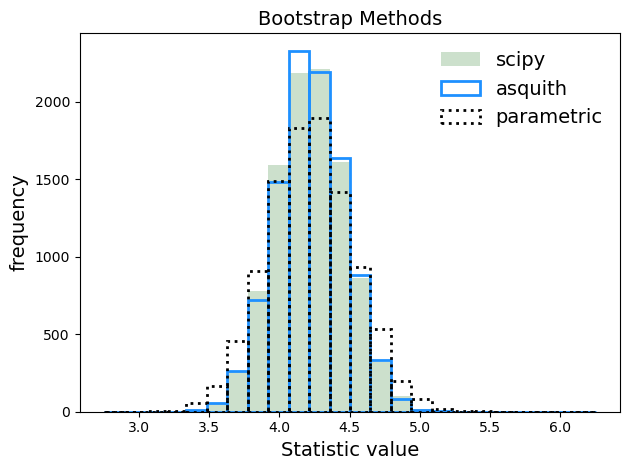
\includegraphics[scale=0.33]{bootstrap.png}
\end{center}
\scriptsize
\rbl{*This uncertainty was the highest returned by the three methods, so I went with it to be conservative. If I ran again without a seed, a different method would be highest. Random!}
\end{frame}


\begin{frame}[fragile]{Variations on the Bootstrap}
\small
There are uncountable variations on this technique. One handy one is 'smoothing':\\

\scriptsize
\begin{minted}[bgcolor=LightGray]{python}
noisy_sigmas=[]
for i in range(9999):
	bs=[ np.random.choice(sample, replace=True) for j in range(100)] 
	noisy_std = norm(np.std(bs),0.5).rvs()	
	noisy_sigmas.append( noisy_std )

noisy_ser=f'{np.std(noisy_sigmas):.2f}'
noisy_cv=f'{np.mean(noisy_sigmas):.2f}'
print( f'Noisy bootstrap: {noisy_cv}+/-{noisy_ser}')	
# Noisy bootstrap: 4.22+/-0.56
# regular bootstrap: 4.23+/-0.25
\end{minted}
\end{frame}

\begin{frame}[fragile]{Variations on the Bootstrap}
\small
Smoothing: \magtn{adding noise to the sample inflates the uncertainty but does not alter the mean.}\\

\begin{center}
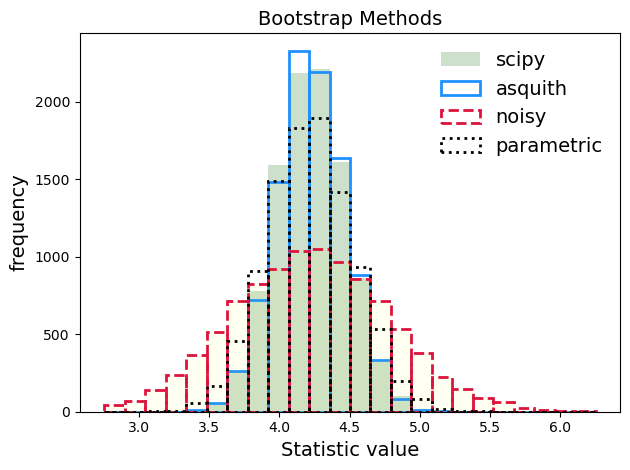
\includegraphics[scale=0.45]{nbootstrap.png}
\end{center}
\end{frame}

\section{MCMC}

\begin{frame}{Back to Bayes!}
\Huge
\begin{center}
 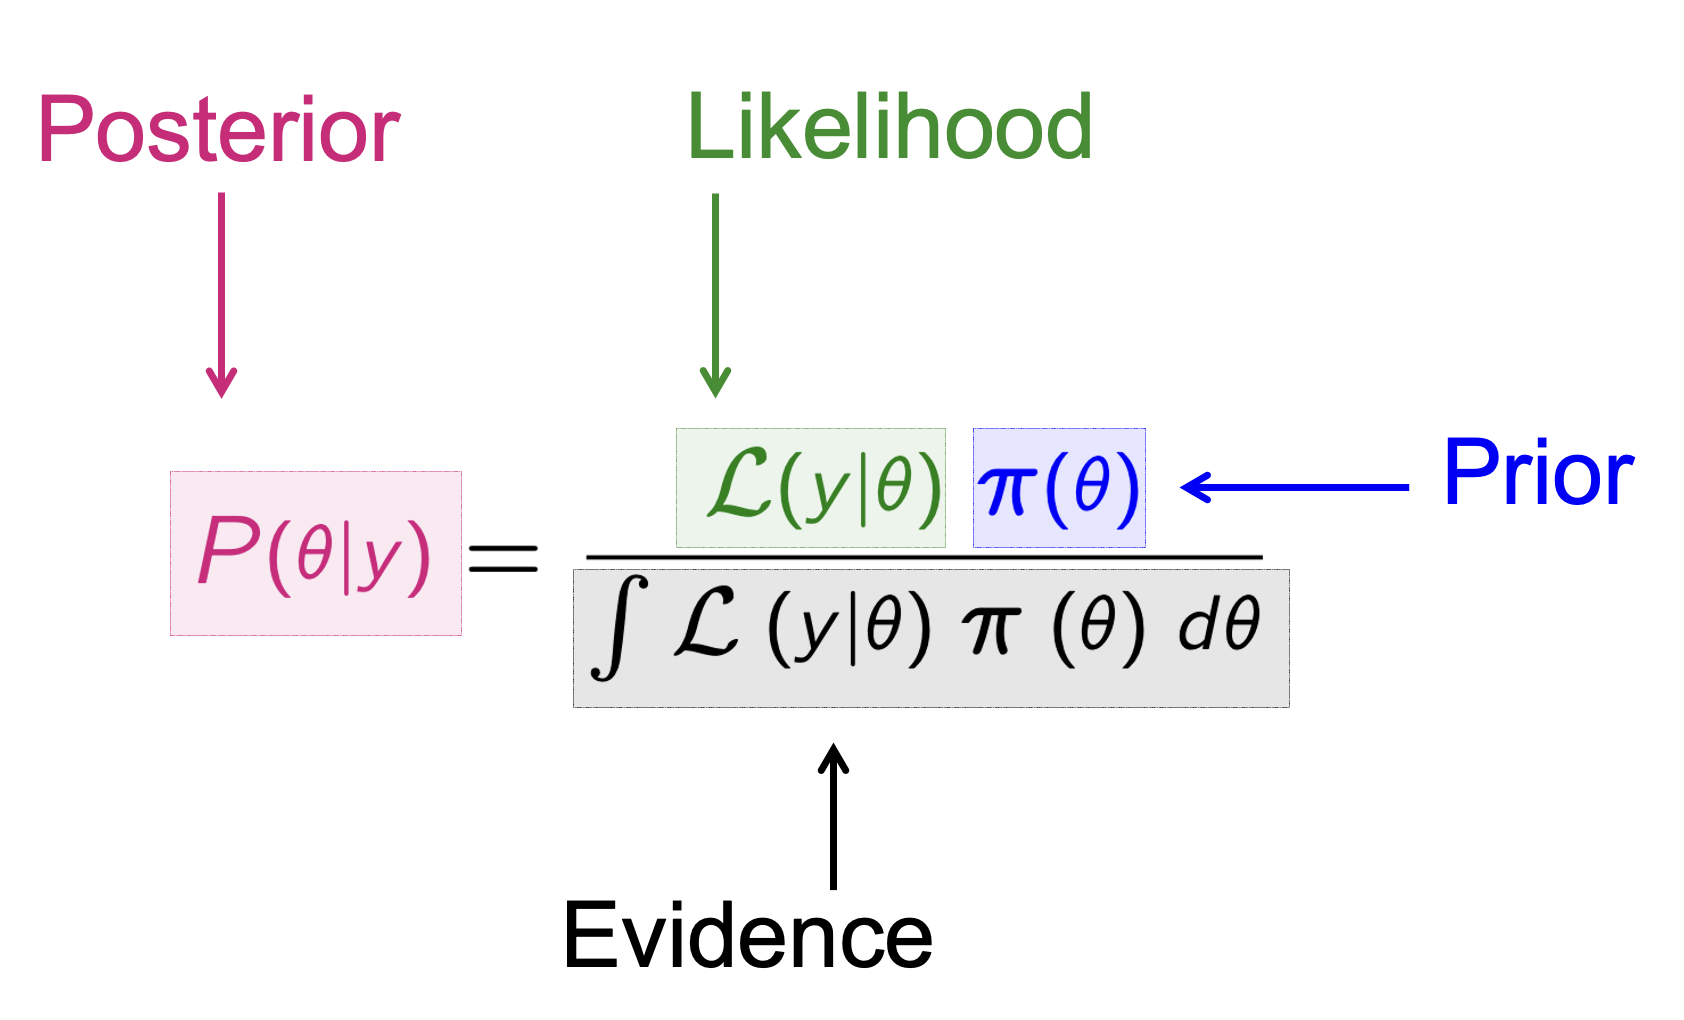
\includegraphics[scale=0.3]{BayesPic.png}
\end{center}
\end{frame}

\begin{frame}{We looked at Poisson-Gamma}
\small
Gamma priors:  \bbl{$\pi(\theta) \propto  \theta^{\alpha-1} e^{- \beta \theta}$}\\[1ex]
Poisson likelihoods: \gbl{$\mathcal{L}\wee{(y|\theta)}  \propto \theta^{n\,\overline{y}}  e^{-n\theta}$ }\\[1ex]
Gamma Posterior: \magtn{$Gamma(\alpha+n\overline{y}, \beta+n )$}\\[1ex]

%Posterior is Gamma($\alpha',\beta'$) with $\alpha' = \alpha+ n\overline{y}$ and $\beta' = \beta+ n$:\\[1ex]
%\magtn{$P(\lambda|y) \propto  \lambda^{\alpha+ n\overline{y} -1  } e^{-(\beta+n) \lambda}$}\\[1ex]

Note that for Gamma, the \rbl{Expected Value} is $E[\theta]= \alpha \beta$ and the \rbl{Variance} is $V[\theta]= \alpha \beta^2$\\[1ex]

Compare with Poisson $E[y]= \theta$ and $V[y]= \theta$\\[1ex]

For example, if we have Poisson data and guess at the rate parameter $\theta = 15$, we want $\alpha \beta = 15$ and $\alpha \beta^2 =  15$ ie $\alpha=15, \beta=1$.\\[1ex]
%We will use this for credible interval example.

\end{frame} 

\begin{frame}{Poisson-Gamma: \small$\magtn{Gamma(\bbl{\alpha}+}\gbl{n\overline{y}}\magtn{, \bbl{\beta}+}\gbl{n}\magtn{ )}  \propto \gbl{ \mathcal{L}(Data | \theta=15) } \times  \bbl{Gamma(\alpha, \beta)}   $}
\small
We saw that the analytical Posterior \magtn{$P(\theta|y)$} does a great job at converging on the mean value of $\theta$, and the MAP estimate $\hat{\theta}$ is the mode of the Posterior.
\begin{center}
 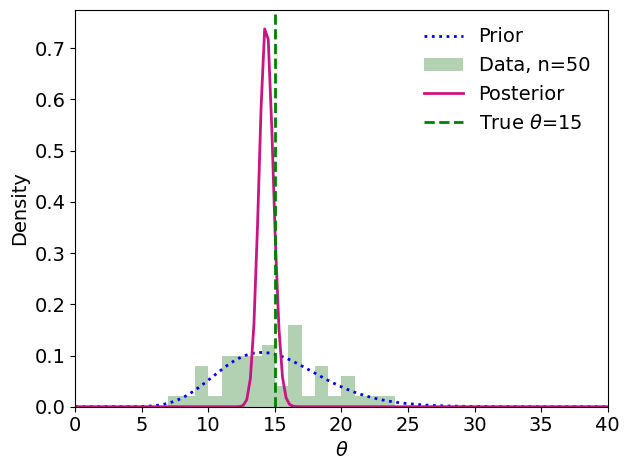
\includegraphics[scale=0.5]{hnPG-a15-b1-n50.png}
\end{center}
\end{frame} 

\begin{frame}{Poisson-Gamma}
\small
Then it was Wednesday evening and we all tried to stay awake while I introduced the Predictive Posterior.
\begin{center}
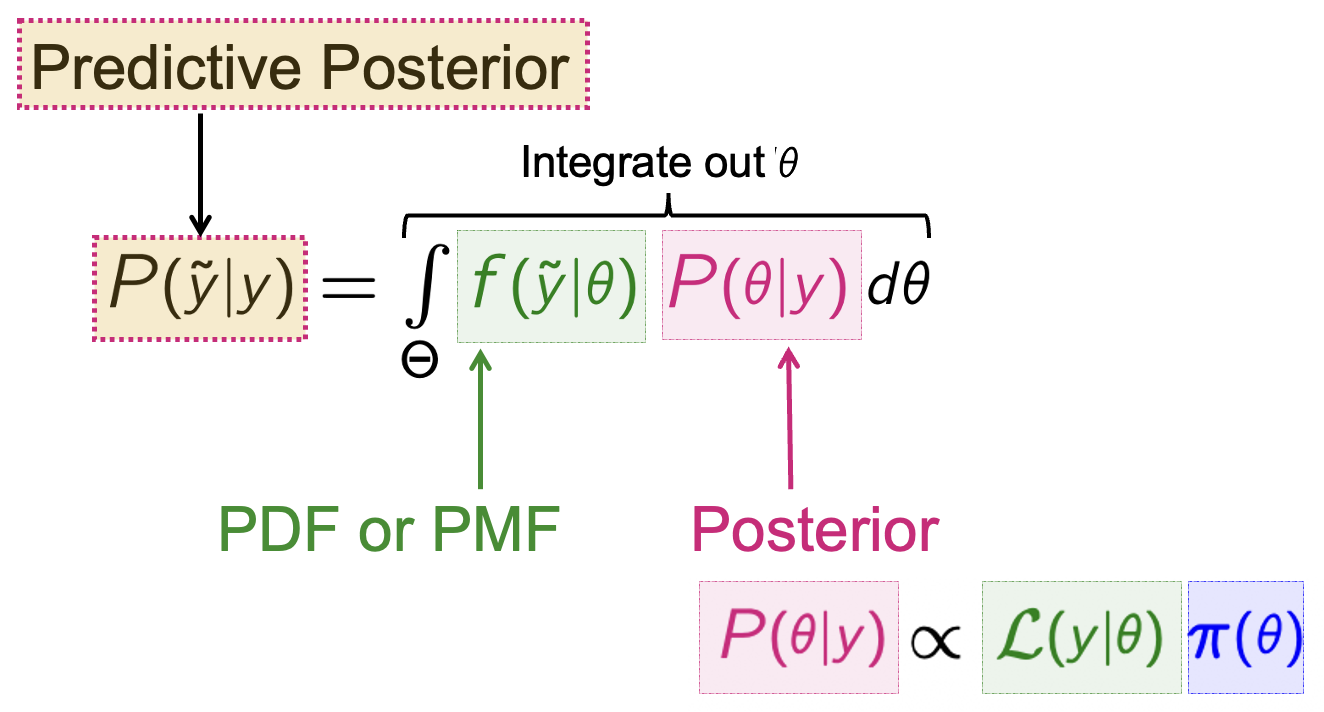
\includegraphics[scale=0.45]{predD.png}
\end{center}
\end{frame} 


\begin{frame}{Poisson-Gamma}
\small
For Poisson-Gamma the Predictive is a negative binomial. It is awesome because we get the whole distribution as prediction rather.% than just the most probable value.
\begin{center}
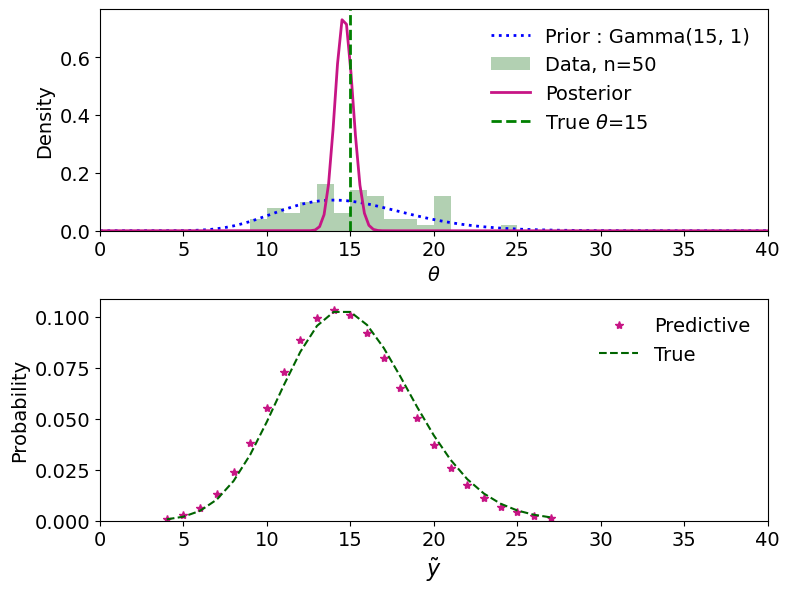
\includegraphics[scale=0.35]{predPG-a15-b1-n50.png}
\end{center}
\end{frame} 




\begin{frame}{MCMC}
\small
The workshop problem / python example for last week will have showed you the process of building an analytical Predictive posterior.\\[1ex]

\magtn{If it is not possible to construct an analytical Predictive Posterior, we can approximate one using MCMC.}\\[1ex]


To use MCMC we construct the Posterior from the Likelihood and the Prior (which can be uninformative, for example Uniform).\\[1ex]

Then we 'fill out' a Sampling distribution. We start at some random parameter value, and take random steps around the parameter space. \\[1ex]

The sequence of random steps is called a Markov Chain. \\
\end{frame}

\begin{frame}{Plot from Poisson-Gamma Example}
\small
\begin{center}
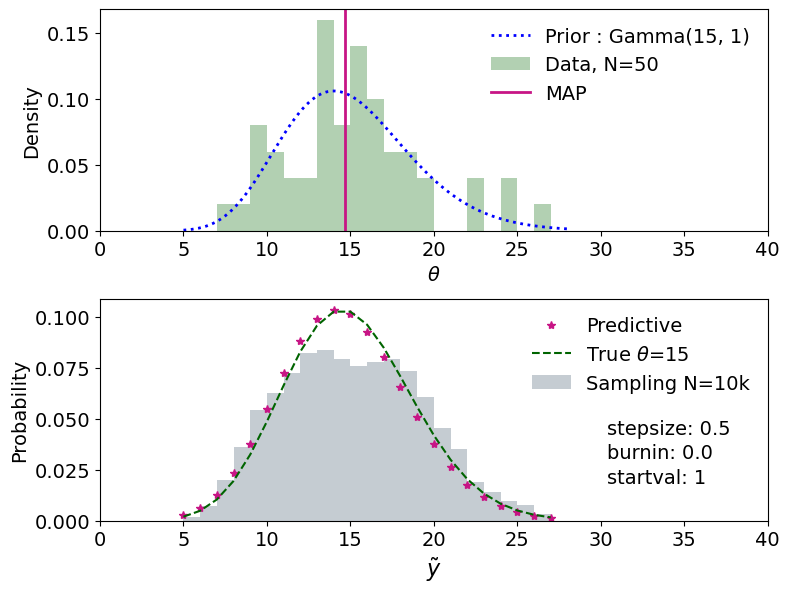
\includegraphics[scale=0.45]{Fig-PoisGam-a15-b1-n50-step0.5-burn0.0-guess1-nsamp10000-1765153696.png}
\end{center}
\end{frame}

\begin{frame}{MCMC}
\small
\bbl{At each step in the Markov Chain we ask:}\\

\magtn{Is the Posterior for this value $y=\theta_1$ larger than the Posterior for the previous data value $y=\theta_0$?}\\

\ghl{Yes!}: Put this new data value $y=\theta_1$ in a container to include as part of our distribution.\\[1ex]
\yyhl{\rbl{No.}}: Roll a dice and decide whether to include it or not.\\[1ex]

\bbl{Then we take another step.}\\[1ex]

The decision at each step depends only on the posterior probability calculated at the previous step, so this sequence gets the privilege of being called a Markov Chain. \magtn{It is memoryless.}


\end{frame}


\begin{frame}{Metropolis Hastings}
\small
\bbl{The example I have provided in  \texttt{PoissonGamma.py} uses Metropolis Hastings}.\\[1ex] 

One Metropolis Hastings iteration looks like this:\\[1ex]
1. Starting value (guess)\\[1ex]
2. Add random noise to guess\\[1ex]
3. Compare Posteriors, and if the new guess is better, we stick with it. If the new guess is worse, we may still keep it- we assign a probability to it depending on how much worse it is.\\[1ex]
Then we repeat. Each iteration is independent of the one before.\\[1ex]

\magtn{ What if we have more than one parameter to estimate?}
\end{frame}



\begin{frame}{Gibbs}
\small
\bbl{Gibbs sampling is a version of Metropolis that can handle multiple parameters:}\\[1ex]

1. Start with a pair of guesses for a pair of parameters: a,b.\\[1ex]
2. Add random noise to the guess for a.\\[1ex]
3. Compare Posteriors, GIVEN b, and if the new guess is better, we stick with it. If the new guess is worse, we may still keep it- we assign a probability to it depending on how much worse it is.\\[1ex]
Then repeat this 3-step process for b given a.\\[1ex]

\magtn{ This can be super-slow. Differential Evolution is our friend.}\\[1ex]
\end{frame}


\begin{frame}{Differential Evolution}
\small
\bbl{All the cool kids use Differential Evolution!}\\[1ex]


Differential Evolution starts with a set of many initial guesses, and generates one chain of samples from each initial guess.\\[1ex]
%The chains can 
%
%Instead of starting with a single guess and generating a single chain of samples from that guess, DE starts with a set of many initial guesses, and generates one chain of samples from each initial guess. These multiple chains allow the proposals in one chain to be informed by the correlations between samples from the other chains\\
1. Starting value (guess) for chain 1 \\[1ex]
2. Randomly select a pair of other chains and use the difference in the value between them, $\Delta$ (multiplied by a tuning parameter) as the noise. Then add a small amount of random noise (to avoid degeneracy).\\[1ex]
3. Usual deal for step 3!\\[1ex]

%This is nice because it only has two tuning parameters, one for the scale and one for the small amount of random noise. Normal MH has a separate tuning parameter for every model parameter.\\
\end{frame}

\begin{frame}{Probabilistic Programming Libraries}
\small
PyMC is probably the most widely used. \href{https://www.pymc.io/welcome.html}{Docs} are a bit opaque, but we live at a fine time for progress on that front.\\[1ex]

The emcee library is very easy and is popular with astronomers, but as far as I can tell it is not possible to make Predictive distributions, which seems a bit of a shame. \href{https://emcee.readthedocs.io/en/stable/tutorials/quickstart/}{Docs here}.\\[1ex]

I expect you have instruction in these things if you are going into ML. In case you are not expecting that in your future but want to play with the toys, this looks like an excellent introduction using pymc:

\href{https://nbviewer.org/github/CamDavidsonPilon/Probabilistic-Programming-and-Bayesian-Methods-for-Hackers/blob/master/Chapter1_Introduction/Ch1_Introduction_PyMC2.ipynb}{Bayesian-Methods-for-Hackers}.\\

\magtn{Last lecture Wednesday: Tuning!}
\end{frame}



%
%\begin{frame}[fragile]{Tuning}
%\small
%The parameters for the 'by-hand' python example I have provided are:\\[1ex]
%
%\scriptsize
%\begin{minted}[bgcolor=LightGray]{python}
%# SAMPLING HYPERPARAMETERS
%s_N=5_000       # Number of samples. More is more.
%s_guess=-1      # Starting value (-1 means choose randomly from data range)
%s_stepsize=5    # Max amount of smearing from the starting value
%s_burnin=0.1    # Fraction of samples to use for burning in the sampler
%\end{minted}
%
%\end{frame}
%
%
%\begin{frame}[fragile]{Tuning: Number of Samples}
%
%\scriptsize
%\begin{minted}[bgcolor=LightGray]{python}
%s_N=5_000      # Number of samples. More is more.
%\end{minted}
%
%Figures showing effect of increasing number.
%\end{frame}
%
%
%
%\begin{frame}[fragile]{Tuning: Starting Value and Step Size}
%
%\scriptsize
%\begin{minted}[bgcolor=LightGray]{python}
%s_guess=-1      # Starting value (-1 means choose randomly from data range)
%s_stepsize=0.5    # Max amount of smearing from the starting value
%\end{minted}
%
%We can check on our choice of step size by looking at a Trace Plot:\\[1ex]
%\begin{center}
%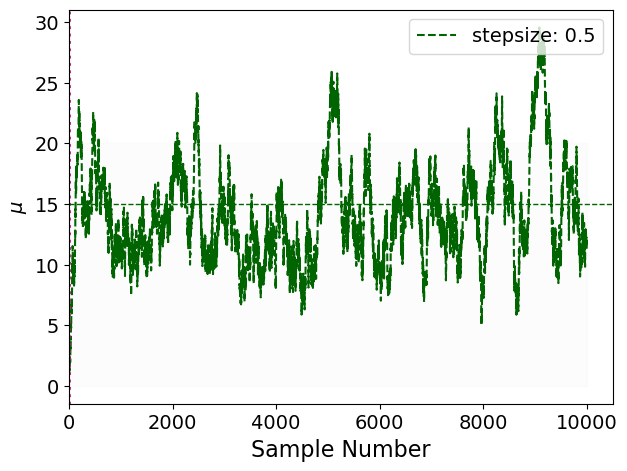
\includegraphics[scale=0.25]{Fig-PoisGam-Trace_stepsize0.5.png}
%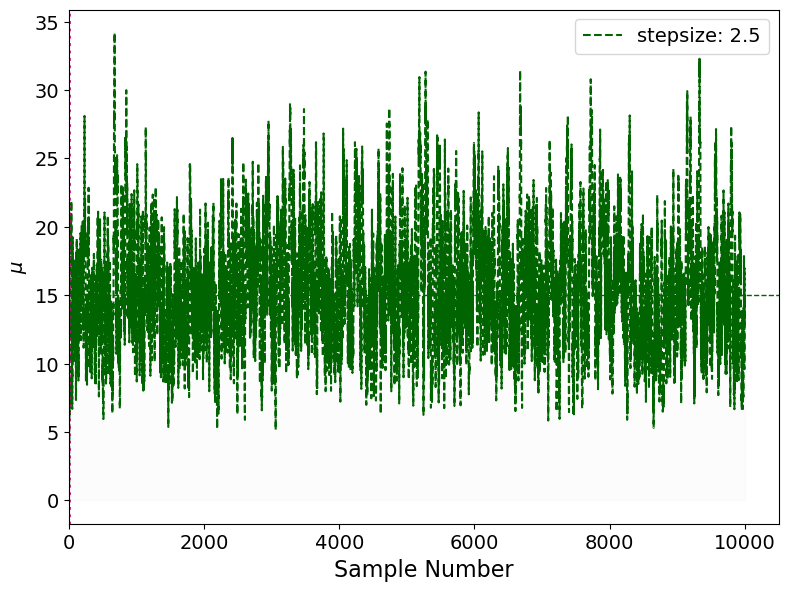
\includegraphics[scale=0.25]{Fig-PoisGam-Trace_stepsize2.5.png}
%\end{center}
%The right hand plot with the larger step size is the better choice here because it is not hyperfocusing on lots of detailed fluctuations in probability, and is covering the true parameter value well.
%\end{frame}
%
%
%\begin{frame}[fragile]{Tuning: Burn-in}
%
%\scriptsize
%\begin{minted}[bgcolor=LightGray]{python}
%s_burnin=0.1    # Fraction of samples to use for burning in the sampler
%\end{minted}
%
%
%\end{frame}

%\begin{frame}{Markov Chains}
%\small
%
%The first steps of a Markov Chain are susceptible to being problematic, because we start at some random point for which there may be tiny probabilities for all values tested, but because we only care about the ratio of probabilities between this one and the last one, we will be accepting all sorts of trash.\\[1ex]
%
%\end{frame}








%\begin{frame}{Important things to get right}
%\small
%The Posteriors we use must be properly constructed, so that their relative values are meaningful.\\[1ex]
%
%We don't need the analytical form of the posterior to do this, we just need to recalculate the log likelihood and the prior for every point, then multiply them together. We are using numerical values.\\
%
%
%\end{frame}
%
%
%
%\begin{frame}{Ensuring Memorylessness}
%\small
%The randomness is introduced
%
%\rbl{Autocorrelation}
%\end{frame}
%
%
%\begin{frame}{What on earth is this?}
%\small
%Trace plot. Often devoid of any useful information, yet universally popular.
%
%\end{frame}
%
%
%
%\begin{frame}{First Steps: The Burn-in}
%\small
%
%
%\end{frame}
%\begin{frame}{MCMC}
%\small
%If we can produce the predictive posterior analytically, then we should! This is because it is the best possible solution.
%If we can't, then we have the option of using markov chains.
%Note that we still have to start with the posterior.
%For example when we looked at Poisson Gamma last week we found that the Posterior is
%Gamma(α+ ny, β+ n)
%Prior: Gamma(α, β)
%Poisson Likelihood with guess θ= 15
%α= 15, β= 1
%Prior: Gamma(15, 1)
%The posterior then changes its form with every data point we add,
%Gamma(α+ ny, β+ n)
%because n is the number of data points and y is the mean value
%We then saw that we can make a predicitve posterior analytically in this case, and it is negative binomial
%nbinom(α+ ny, (β+ n)/(β + n + 1) )
%P(y'|y) = integral f (y' |θ) P(θ|y ) d θ
%This allowed us to "fill out" our posterior because we now have integrated out the parameter and are just modelling the data. This is why the predictive has a distribution, whereas the posterior just spikes around the most likely value of the parameter. The predictive is a sampling distribution for our data.
%
%What if we couldn't do this? We are able to use this in the workshop example because I looked up the proof.
%We would take our posterior Gamma(α+ ny, β+ n) and use it generate samples, by trying slightly altered parameters and calculating their relative likelihoods with respect to our starting parameters.
%\end{frame}



%
%\begin{frame}{Bayes Factors}
%\small
%\end{frame}



\begin{frame}{Thanks For Your Time}
\center
\Huge
Fin.
\end{frame}

\end{document}



